
\begin{frame}[c]\label{c.1}
\frametitle{A Theory of Onset Temperature in 2D: The Mean-Squared Displacement}


\begin{columns}[T]
\begin{column}[T]{0.4\textwidth}
\vspace{-12pt}
\begin{figure}[t]
%\includegraphics[height=0.65\textheight]{figures/pel_hopping.png}
\begin{overprint}

\onslide<3>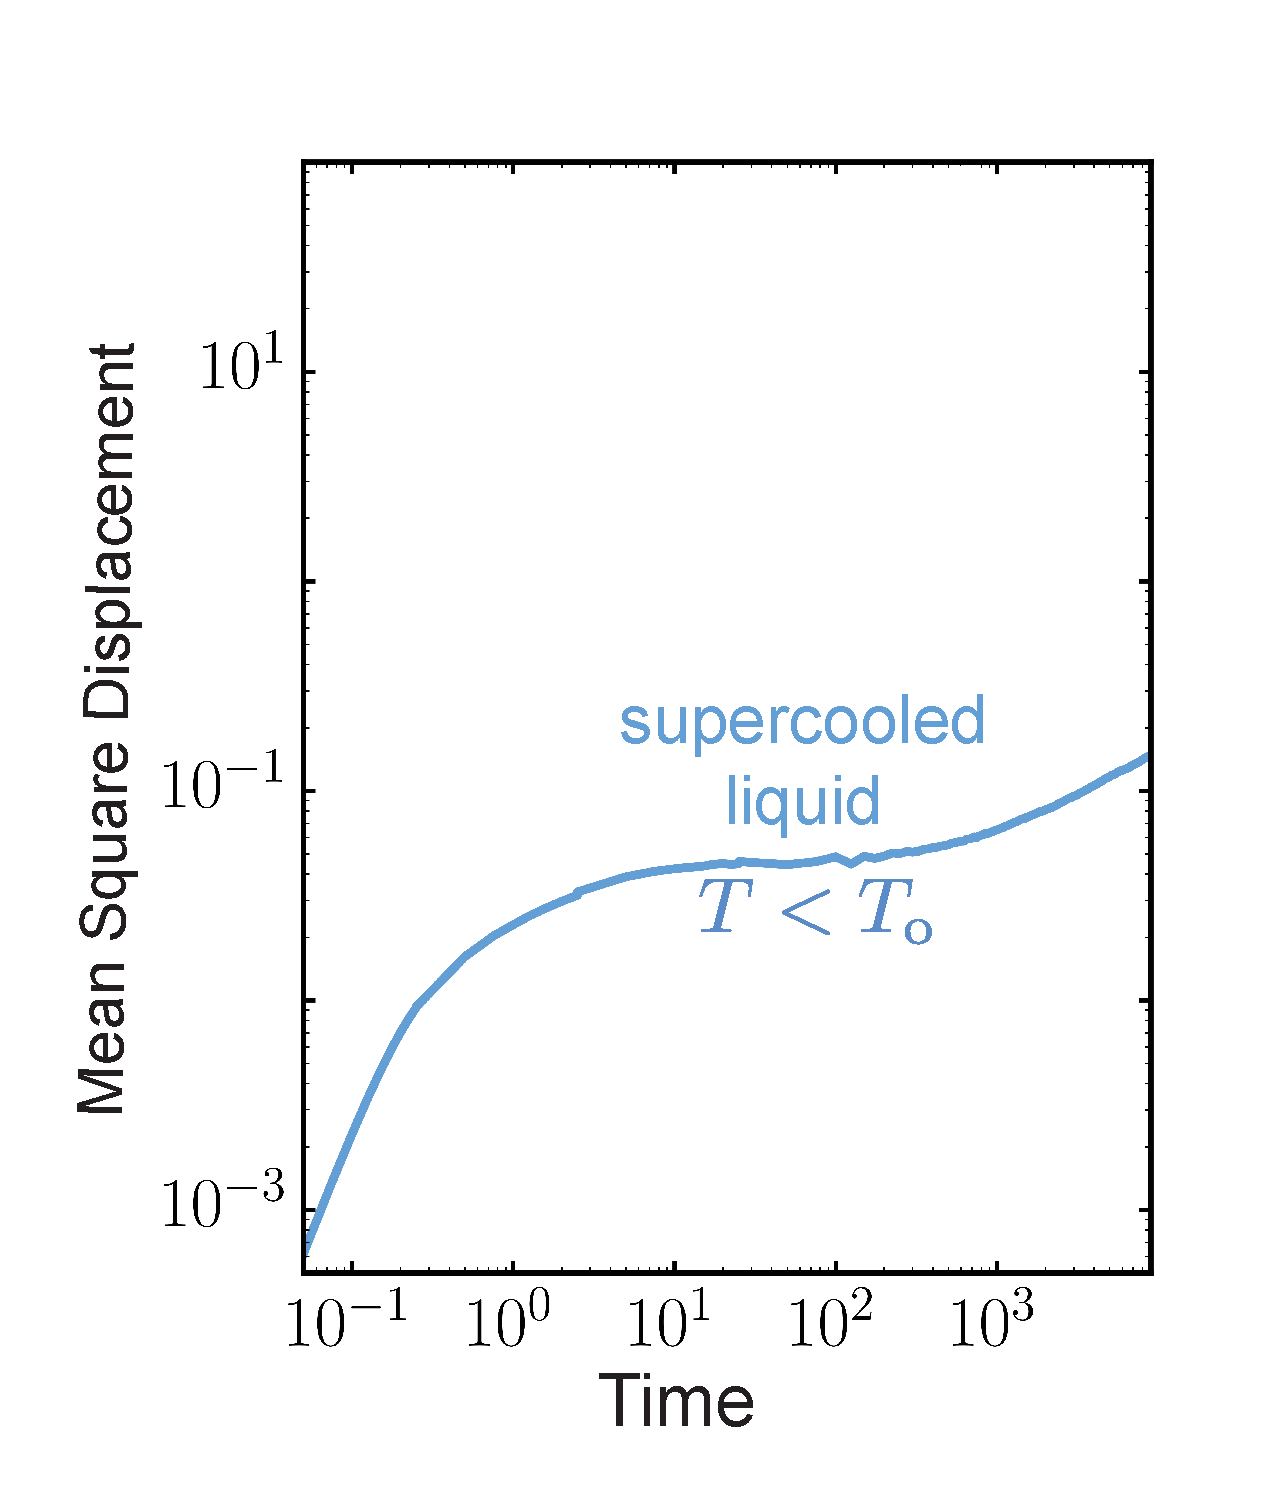
\includegraphics[height=0.75\textheight]{c.1-kt_msdintro/msd-supercooledliq-0.pdf}\caption{The MSD of a polydisperse system at $ T \approx 0.50 T_\mathrm{o}$}


\onslide<4-5>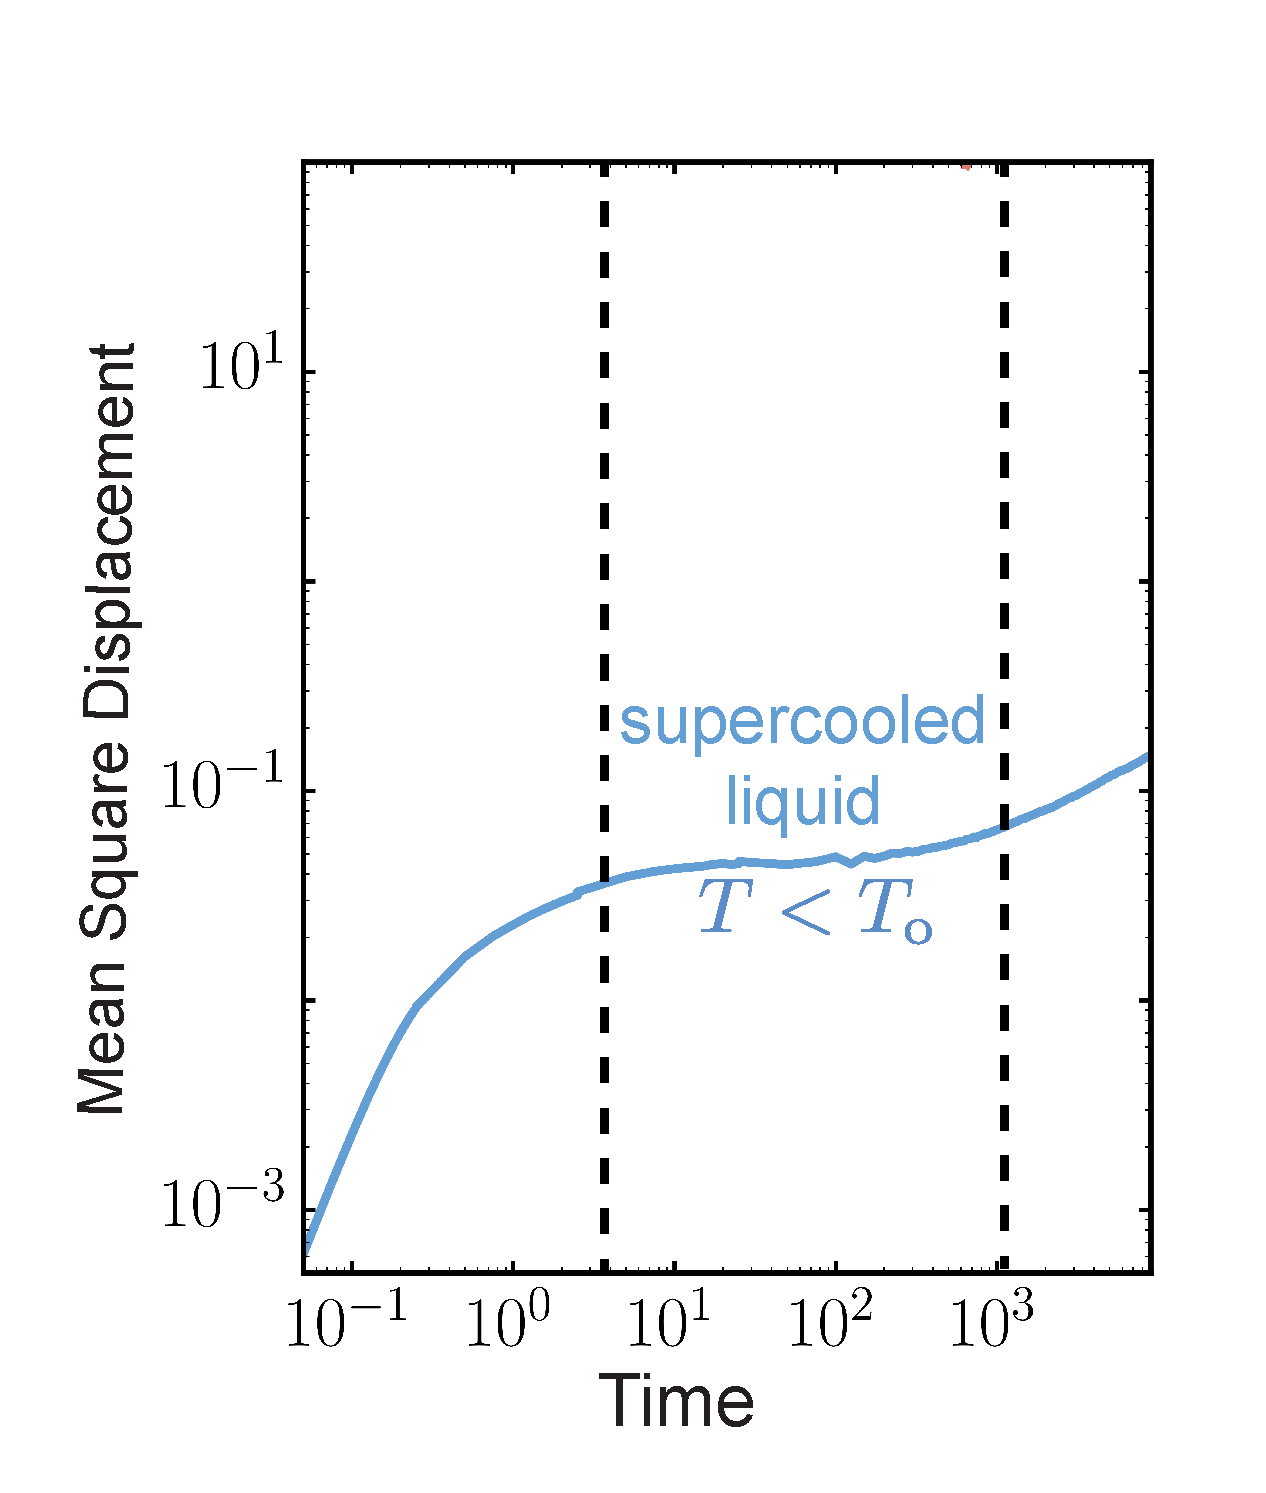
\includegraphics[height=0.75\textheight]{c.1-kt_msdintro/msd-supercooledliq-1.pdf}\caption{The MSD of a polydisperse system at $ T \approx 0.50 T_\mathrm{o}$}

\onslide<6>\includegraphics[height=0.75\textheight]{c.1-kt_msdintro/msd-supercooledliq-2.pdf}\caption{The MSD of a polydisperse system at $ T \approx 0.50 T_\mathrm{o}$ with snapshot of excitation events (in yellow)}


%\onslide<7>\includegraphics[height=0.75\textheight]{c.1-kt_msdintro/msd-supercooledliq-3.pdf}\caption{The MSD of a supercooled liquid $ T \approx 0.50 T_\mathrm{o}$ with snapshot of excitation events (in yellow)}


\onslide<7>\includegraphics[height=0.75\textheight]{c.1-kt_msdintro/msd-supercooledliq-4.pdf}\caption{The MSD at high temperatures $T \approx 2.0 T_\mathrm{o}$}


\onslide<8->\includegraphics[height=0.75\textheight]{c.1-kt_msdintro/msd-supercooledliq-5.pdf}\caption{The MSD at high temperatures $T \approx 2.0 T_\mathrm{o}$ with snapshots of mobile regions (in yellow)}


\end{overprint}
\end{figure}


\end{column}

\begin{column}[T]{0.6\textwidth}



\only<2->{Observe the mean-squared displacement (MSD) of a particle}
\begin{enumerate}
\item<4-> $T < T_\mathrm{o}$: ``Plateau" region\uncover<5->{, shearing yields \textbf{solid} behavior}\uncover<6->{, filled with \textbf{rare excitation events}} %$t \sim \langle \tau_\mathrm{jump} \rangle \ll \langle \tau_\mathrm{eq} \rangle$)
\item<7-> $T > T_\mathrm{o}$: Immediate diffusion, shearing yields \textbf{fluid} behavior\uncover<8->{, populated with \textbf{many mobile regions}.} 
\end{enumerate}

\onslide<9->{\begin{block}{\centering \large Origin of Onset Temperature}
\onslide<10->{\centering Onset of glassy dynamics is linked to a "melting" transition at intermediate timescales $t \ll \tau_\mathrm{eq}$}


\onslide<11->{\centering An elastic solid $ \leftrightarrow $ a fluid

%At intermediate timescales ($t \sim \langle \tau_\mathrm{jump} \rangle \ll \langle \tau_\mathrm{eq} \rangle$)
}
\end{block}

}

\vspace{10pt}

\km{\onslide<12->{\centering \Large What is the mechanism for the "melting" transition?}}

\end{column}
\end{columns}



\end{frame}

